\paragraph{Paneles de Absorción}

\paragraph{Paneles de difracción}
Los paneles de difracción están caracterizados por su capacidad de reflejar las ondas de sonido en muchas direcciones, lo que permite una mejor distribución de la energía acústica en el cuarto. Los difusores permiten que los oyentes reciban muchas mas reflexiones de menor energía y que por tanto, tengan una mayor sensación de profundidad y de volumen. \cite{PilchDiffusers}\\
Existen diversos tipos de difusores, a continuación se listan los mas importantes \cite{TypesDiffusers}:
\begin{itemize}
    \item Difusores de tipo \textit{Skyline}. Consta de agrupaciones de bloques a diferentes alturas que recuerdan a los rascacielos de una ciudad (De ahí su nombre). Las diferentes alturas permiten que las ondas reboten en diferentes instantes del tiempo, además, la diferencia en la dirección de las superficies permite que se reflejen hacia diversas direcciones.
    \item Difusores de residuo cuadráticos. Consta de diferentes canales que corren paralelos en el panel, a diferentes profundidades. Las profundidades no son aleatorias, sino que están diseñadas para ser eficientes a ciertas frecuencias.
    \item Difusores de residuo cuadráticos en 2D. Son muy similares a los de tipo \textit{Skyline} con la diferencia que están cuidadosamente planificados para ser eficientes a ciertas frecuencias, además, los bloques se separan entre ellos.
    \item Difusores de barril. Se asemejan a un cilindro cortado a la mitad, y se colocan convexos al cuarto. Su geometría permite reflejos especulares que varían de acuerdo al punto de impacto. Se diferencian del resto por su capacidad de albergar materiales absorbentes en el interior, lo que permite absorber frecuencias que no se difractan. 
    \item Difusores piramidales. Constan de pirámides cuadrangulares de diferentes alturas, lo que modifica los angulos de incidencia.
\end{itemize}
Para nuestra aplicación, se decidió utilizar los Difusores de residuo cuadrático (también llamados \textit{Schoroeder Diffusers} o QRD), ya que, además de permitirnos atacar ciertas frecuencias importantes para nosotros, también son fáciles de manufacturar. 
La sección transversal de un panel QRD es la siguiente \cite{PilchDiffusers}:
\begin{figure}[!htb]
    \centering
    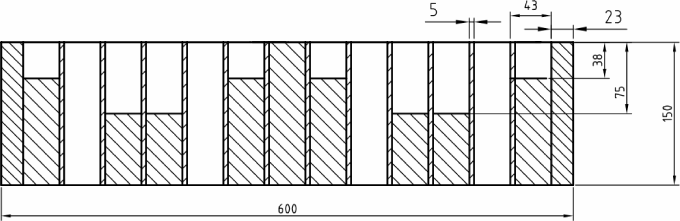
\includegraphics[width=0.8\textwidth]{imagenes/QRD-150-diffusers-cross-section.png}
    \caption{Sección transversal de un panel QRD}
    \label{fig:QRDCross}
\end{figure}
\FloatBarrier
La manufactura constará de una operación con la fresadora para realizar cada uno de los canales a partir de un bloque solido, la altura de la fresadora se ajustara para las diferentes profundidades. \\
Los paneles QRD pueden colocarse paralelos o rotados 90 grados uno respecto del otro. Si se colocan todos paralelos, la difraccion de las ondas ocurrirá solamente en el eje perpendicular a la dirección de los canales. La rotación de los difusores QRD permite que las ondas sea difractados en ambos ejes.